\documentclass{article}
\usepackage{geometry}
 \geometry{
 a4paper,
 total={170mm,257mm},
 left=20mm,
 top=20mm,
 }
\setcounter{section}{-1} % start with the first section (objective) at 0
\usepackage{graphicx}
\usepackage{caption}
\usepackage{booktabs}
\usepackage{hyperref}
%\usepackage{minted}    % VHDL support

\title{\LARGE Testing and fault tolerance\\ \textbf{\huge }\\ \Large Technical report \vspace*{0.3in}   }
\author{Samuele Yves Cerini, s256813\\
        Federico Pozzana, s254758 \\
\textbf{Professor} Matteo Sonza Reorda \vspace*{2.0in}}
\date{January 16, 2020}

\begin{document}
\pagenumbering{gobble}
\thispagestyle{empty}

\begin{figure}
    \centering
    
\includegraphics[scale=0.1]{PoliLogo.png}
    \captionsetup{labelformat=empty}
    \caption {\LARGE Politecnico di Torino}
\end{figure}

\maketitle
%\newpage

\pagenumbering{arabic}
\thispagestyle{empty}
\tableofcontents
\newpage

%   _____  _____   ____       _ ______ _____ _______    ____  ____       _ ______ _____ _______ _______      ________
%  |  __ \|  __ \ / __ \     | |  ____/ ____|__   __|  / __ \|  _ \     | |  ____/ ____|__   __|_   _\ \    / /  ____|
%  | |__) | |__) | |  | |    | | |__ | |       | |    | |  | | |_) |    | | |__ | |       | |    | |  \ \  / /| |__
%  |  ___/|  _  /| |  | |_   | |  __|| |       | |    | |  | |  _ < _   | |  __|| |       | |    | |   \ \/ / |  __|
%  | |    | | \ \| |__| | |__| | |___| |____   | |    | |__| | |_) | |__| | |___| |____   | |   _| |_   \  /  | |____
%  |_|    |_|  \_\\____/ \____/|______\_____|  |_|     \____/|____/ \____/|______\_____|  |_|  |_____|   \/   |______|
%
%

\section{Project objective}
The objective for this assignment is to develop a functional testbench in the form of a single program, either written in \texttt{C} or in \texttt{asm}, able to target single transition delay faults for the execution unit of a \emph{RISCY} CPU. Some assumptions made for this project are:
\begin{itemize}
    \item Single transition delay faults
    \item I/O signals observable and controllable at any clock cycle
\end{itemize}
The default flow provided during the lab sessions has been used, only the \texttt{tmax.tcl} file has been modified to evaluate the faults in the execution unit and to look for delay faults instead of stuck-at faults.

%             _____ __  __
%      /\    / ____|  \/  |
%     /  \  | (___ | \  / |
%    / /\ \  \___ \| |\/| |
%   / ____ \ ____) | |  | |
%  /_/    \_\_____/|_|  |_|
%
%

\section{ASM program}
In order to achieve a low execution time (thus keeping the entire test-phase as fast as possible) we decided to make use of the \emph{RISCV} assembly language. This decision also allowed us to manipulate each instruction of the processor at a finer grain as we will explain further in this report. Finally, using the assembly language allowed us to follow the exact same flow involving the use of \emph{TetraMAX}'s \emph{ATPG} functionalities, as done previously in one of the course's labs (lab \#4).
The assembly program developed for this assignment can be divided into three macro categories, namely:
\begin{itemize}
    \item ATPG generated instructions
    \item LFSR-like generated instructions
    \item LAB4-based generated instructions
\end{itemize}
All the assembly files generated have been included into the provided \texttt{main.S} assembly program. We will now carefully analyze the aforementioned three main categories for our \texttt{asm} files.

At first, we started the evaluation of the execution unit by splitting it into sub-components like the \texttt{ALU} (which also contains the \texttt{DIV} unit) and the \texttt{MUL} unit.
As we can see by looking at the entire \texttt{EXE} fault list the majority of faults (72735 faults in total) is split almost equally between the \texttt{ALU} unit and the \texttt{MUL} unit.

The first approach we used involved the use of \emph{TetraMAX}'s \emph{ATPG}, as we explain in the following section.

%         _______ _____   _____
%      /\|__   __|  __ \ / ____|
%     /  \  | |  | |__) | |  __
%    / /\ \ | |  |  ___/| | |_ |
%   / ____ \| |  | |    | |__| |
%  /_/    \_\_|  |_|     \_____|
%
%

\subsection{ATPG generated instructions}
Hence, we started with the goal to achieve a decent fault coverage for the \texttt{ALU} module. To do that we started by setting a constraint on the \texttt{OPCODE} input signals of the \texttt{ALU} module and let the ATPG to generate automatically all the couples of input patterns. Once the \texttt{.stil} file containing the ATPG's patterns has been produced, we only had to parse it using the same \texttt{python} script provided with lab \#4.

Since the parser was initially intended for \emph{stuck-at faults}, we needed to modify it accordingly: when using the \emph{single-transition delay faults} model, the \texttt{ATPG} generates two distinct \texttt{\_PIs} patterns inside the resulting \texttt{.stil} file. The first pattern is used to excite the fault while the second one is used to propagate it. In order to transmit this behavior also to our assembly program, we needed to modify the parser accordingly. This simple modification is structured as follow: when parsing the first \texttt{\_PI} line of the actual set of \texttt{\_PI + \_PI + \_PO} pattern the goal is to translate this sequence into the corresponding operation (for example, an \texttt{ADD}) between two operand registers (whose value is also parsed from the first \texttt{\_PI} sequence).
The result of this operation is then stored into the stack, altough not strictly necessary since the first \texttt{\_PI} sequence is used to control the fault, not to observe it.

Following the same idea, we parse also the second \texttt{\_PI} sequence into the same operation as before. This time, we must store the value produced into the stack since this value will allow us to observe the transition delay fault.

This approach led to a fault coverage of almost 45\% for the \texttt{ALU} using the majority of the \texttt{ALU}-related instructions (the \texttt{OPCODE} for each operation can be found in the \texttt{riscv\_defines.sv} file).
Many cases and \texttt{ATPG} sessions were made in order to constraint correctly the input signals in order to obtain a increasingly higher fault coverage. As an example: we found that forcing the \texttt{vector\_mode\_i[1:0]} imput signals to the value \texttt{"11"} in order to enable the 8-Bit vector mode (to perform four operations on the 4 bytes inside a 32-bit word at the same time) led us to a similar fault coverage to the one obtained with the vector mode disabled but with a lower number of patterns produced. This allowed us to obtain up to $2x \div 3x$ improvement on the total execution time.

Finally, we decided to build a new python script that, given all the \texttt{OPCODE}s of the instructions we wanted to generate \texttt{ATPG} patterns with, could automatically launch \texttt{TetraMAX} for each instruction and parse the provided \texttt{.stil} file into the related \texttt{atpg\_patterns\_\$(OPCODE).S} assembly file. This allowed us to avoiding launching manually \texttt{TetraMAX} for each operation when a minimal modification was made to the constraints or to the parser script.

However, even when we covered the majority of the \texttt{OPCODE}s found in the \texttt{riscv\_defines.sv} file we found that the resulting fault coverage was still not sufficient (i.e. too low), especially considering the huge amount of patterns generated (and the consequent overall test execution time required). Since the overall result was not satisfying enough, we decided to move and test a completely different approach, as explained in the next section.

\subsection{LFSR-like generated instructions}
The following approach we adopted required a complete change of paradigm: we stopped using the \texttt{ATPG} and we started generating patterns using a randomized approach. The first goal was to build a \emph{LFSR-like} assembly program. The program, given two random register values (created manually or using the python-shell \texttt{hex(random.randint(2, pow(2, 32)-1))} command) completes various operations using these two registers, saving the results into the stack, "scrambling" the two operand registers (also using the newly-obtained results for an additional randomization) and finally repeating the process with a new set of instructions, using the freshly scrambled operands.

For each operation, four combinations of the input operands have been tested (where possible):

\begin{itemize}
    \item \emph{Operand1} \texttt{OP} \emph{Operand2}
    \item \emph{Operand2} \texttt{OP} \emph{Operand1}
    \item \emph{Operand1} \texttt{OP} \emph{Operand1}
    \item \emph{Operand2} \texttt{OP} \emph{Operand2}
\end{itemize}

The main idea is to enclose the entire program around a loop that iterates again and again the same operations by always keeping random and different operands registers (as the second iteration will use the scrambled registers obtained when executing the last operations of the first iteration). This approach was applied to all the possible \texttt{ALU}, \texttt{MUL} and \texttt{DIV} operations we found in both the general \emph{RISC-V} Manual and in the \emph{RI5CY} Manual (including nearly-all the custom \emph{RI5CY} instructions).

As we discovered later, this assumption cease to be true after some iterations of the main loop (we found a cap around the fourth iteration of the loop: any additional iteration will have produced additional patterns, of course, but no benefits in terms of fault coverage). This is due to the intrinsic random-resistance property of circuits. Still, this approach led to greatly improved performances in terms of fault coverage, while keeping at the same time a lower number of patterns produced (with respect to the \texttt{ATPG}-based approach) and thus a reduced time needed to complete the fault simulation.

In the following section of code, you can see an example of two operations included into the \emph{LFRS-like} \texttt{MUL} file. Each result is stored into a different stack location. The two input operands \texttt{x18} and \texttt{x19} are finally scrambled using the byte-vectorial \texttt{XOR} operation among the freshly obtained results.

\iffalse
\begin{figure}[!h]
    \centering
    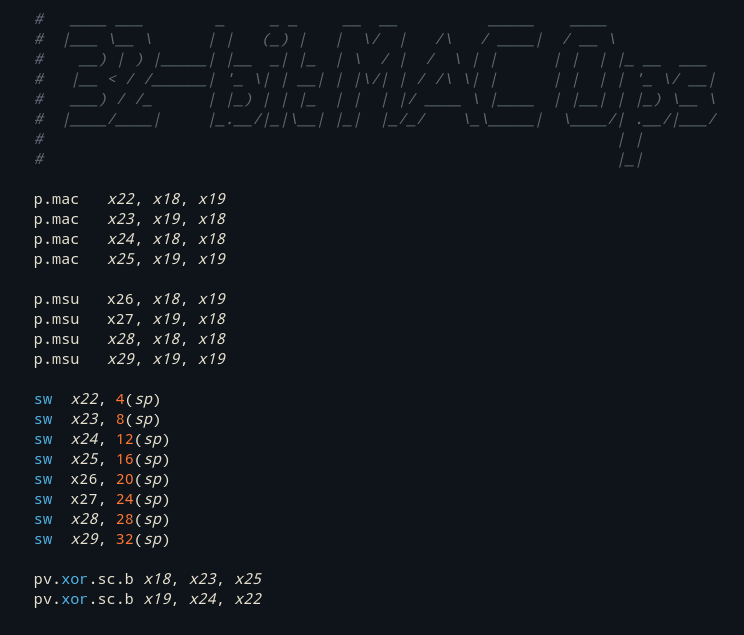
\includegraphics[width=0.6\columnwidth]{./screenshots/lfsrCode.png}
    \caption{Example of two operations included into the \emph{LFRS-like} \texttt{MUL} file. Each result is stored into a different stack location. The two input operands \texttt{x18} and \texttt{x19} are finally scrambled using the byte-vectorial \texttt{XOR} operation among the freshly obtained results.}
    \label{fig:lfsrCode}
\end{figure}
\fi

\begin{verbatim}
    p.mac   x22, x18, x19
    p.mac   x23, x19, x18
    p.mac   x24, x18, x18
    p.mac   x25, x19, x19

    p.msu   x26, x18, x19
    p.msu   x27, x19, x18
    p.msu   x28, x18, x18
    p.msu   x29, x19, x19

    sw  x22, 4(sp)
    sw  x23, 8(sp)
    sw  x24, 12(sp)
    sw  x25, 16(sp)
    sw  x26, 20(sp)
    sw  x27, 24(sp)
    sw  x28, 28(sp)
    sw  x29, 32(sp)

    pv.xor.sc.b x18, x23, x25
    pv.xor.sc.b x19, x24, x22
\end{verbatim}

To overcome the aforementioned limitations due to the increasing resistance to randomization, we had to split the unique file we made for the \texttt{ALU} module into multiple files, with a different internal architecture. Each block that initially composed every single file was in fact copy-pasted 3-4 times inside the same file (in a loop-unrolling fashion): each macro-block of code this time has its set of randomized operands, thus avoiding depending on the previous macro-block of code (for an additional randomization).
This approach has been finally applied only to the files concerning \texttt{ALU} module (that showed a higher resistance to randomization with respect to the \texttt{MUL} and \texttt{DIV} modules.)

This approach finally allowed us to reach the cap of the 80\% fault coverage on the entire Execution Unit.
Due to lack of time we decided to keep the original files with the aforementioned modifications and accepting a fault coverage slightly above the 80\% instead of implementing ex-novo a \emph{Python} script that could solve finally the problem of the random resistance (such script will have completely unrolled the loops, randomizing the two operands after each operation thus requiring no more deterministic scrambling), hence increasing drastically the fault coverage and minimizing the test execution time.


%   _               ____             _  _
%  | |        /\   |  _ \           | || |
%  | |       /  \  | |_) |  ______  | || |_
%  | |      / /\ \ |  _ <  |______| |__   _|
%  | |____ / ____ \| |_) |             | |
%  |______/_/    \_\____/              |_|
%
%

\subsection{LAB4-based generated instructions}
A new approach has also been taken into consideration to further improve the fault coverage obtained with the \texttt{LFSR}-like generated instructions; following the tips provided in the 4th laboratory pdf a loop-based assembly algorithm was implemented, which consists in performing the operation between operands that have a repetition of four by four bits.

Adding the lab4 generated instructions improved the fault coverage by a significant amount without affecting considerably the test time, unlike the \texttt{ATPG} generated instructions.

%   _____  ______  _____ _    _ _   _______ _____
%  |  __ \|  ____|/ ____| |  | | | |__   __/ ____|
%  | |__) | |__  | (___ | |  | | |    | | | (___
%  |  _  /|  __|  \___ \| |  | | |    | |  \___ \
%  | | \ \| |____ ____) | |__| | |____| |  ____) |
%  |_|  \_\______|_____/ \____/|______|_| |_____/
%
%

\section{Results and considerations}

For our final simulation run we decided to abandon completely the patterns obtained with the \texttt{ATPG} and include only the following files (\texttt{LFSR}-like and \texttt{LAB4}-based):

\begin{itemize}
    \item \texttt{ALU (includes \texttt{DIV})}
    \begin{itemize}
        \item \texttt{LFSR\_ALU\_Vect\_Comparison.S}
        \item \texttt{LFSR\_ALU\_General.S}
        \item \texttt{LFSR\_ALU\_Vect\_Ops.S}
        \item \texttt{LFSR\_ALU\_Bit\_Manipulation.S}
        \item \texttt{LFSR\_ALU\_Riscv\_Classic.S}
        \item \texttt{LFSR\_DIV\_Smart\_Patterns.S}
        \item \texttt{LFSR\_DIV\_Unit.S}
    \end{itemize}
    \item \texttt{MUL}
    \begin{itemize}
        \item \texttt{LAB4\_patterns\_mul.S}
        \item \texttt{LAB4\_patterns\_mulh.S}
        \item \texttt{LFSR\_MUL\_Unit.S}
    \end{itemize}
\end{itemize}

By keeping a similar (just slightly modified) approach to our \emph{LFRS-like} allowed us to reach a fault coverage cap that sadly cannot be overcome by just increasing the number of iterations of the assembly program (due to the random-resistance of the logic).
To overcome that cap only a new \emph{python} script with an unrolled approach would have been successful, that sadly we couldn't implement due to time limitations involving the members of this group.
However, as a drawback, such approach based on a python script increases dramatically the code size of the program since no loop is implemented on the assembly side (the entire code is unrolled since this is the only way we found that allows to re-load the operands with completely new and random hexadecimal values after each operation). This must be taken into consideration especially when the memory reserved to code is limited.

Our approach, on the other side, sacrifices a little bit the final fault coverage and the execution time (which is higher with respect to the \emph{completely-unrolled} solution we mentioned above) but heavily reduces the code size (since the loop is actually implemented on the assembly domain).

Both these solutions must be carefully evaluated by the test engineer, considering the final processor he/she has to take into consideration. The three main trade-off parameters that he/she must take into consideration are: fault coverage, test execution time and code size.

Below we report the results obtained with our solution. In the following figure we finally report the fault coverage achieved.

For further references please visit \href{https://github.com/Mrcuve0/TFT-RI5CY-Assignment}{the GitHub Repo (will be made accessible after the project deadline)}.

\begin{itemize}
    \item Patterns generated: 42849
    \item Code size: 147.2 KiB (sbst.hex)
    \item Test time: 10158 seconds
\end{itemize}

\begin{figure}[]
    \centering
    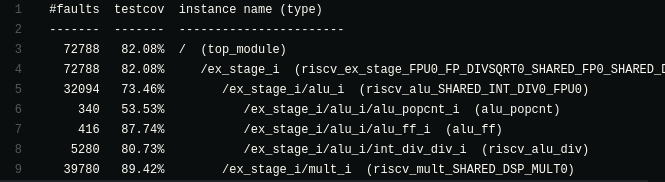
\includegraphics[width=0.6\columnwidth]{./screenshots/faultHierarchy.png}
    \caption{Fault coverage and hierarchy obtained with the final fault simulation.}
    \label{fig:faultHierarchy}
\end{figure}

\end{document}
